\documentclass[letterpaper]{article}
\usepackage[margin=5mm]{geometry}
\usepackage{float}
\usepackage{subcaption}
\usepackage{booktabs}
\usepackage{multirow}
\usepackage{multicol}
\usepackage{graphicx}
\usepackage{paper_commands}

\begin{document}
\thispagestyle{empty} % Remove page number

% maybe pick one of the two relgames figs
\begin{figure}
    \centering
    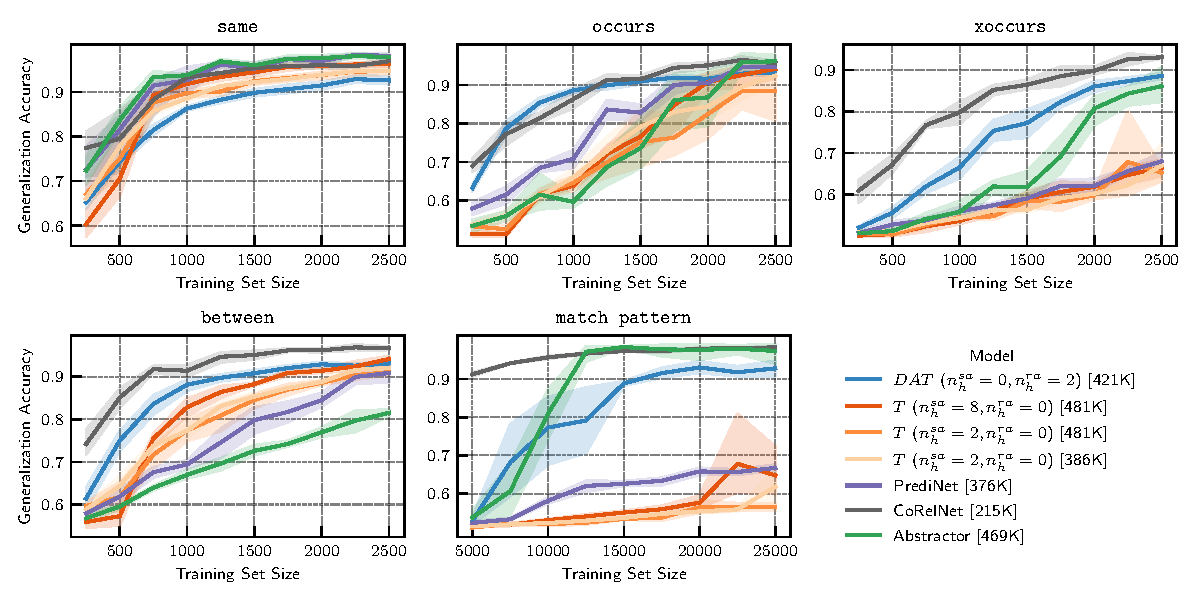
\includegraphics[width=0.8\textwidth]{figs/experiments/relgames/relgames_learning_curves_baseline_comparisons.pdf}
    \caption{Learning curves on relational games, comparing \textit{DAT} against PrediNet, CoRelNet, Abstractor, and Transformer baselines.}
\end{figure}

\begin{figure}
    \centering
    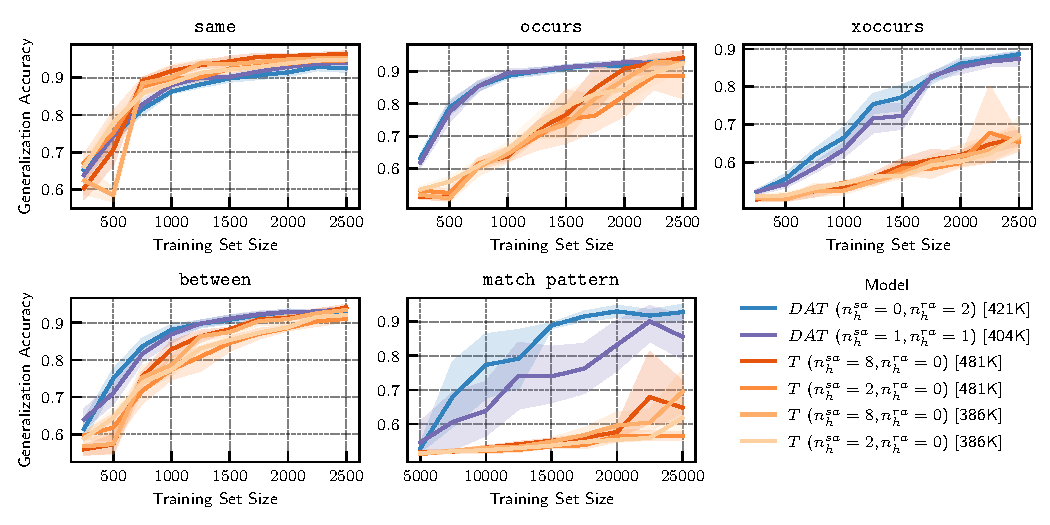
\includegraphics[width=0.8\textwidth]{figs/experiments/relgames/relgames_learning_curves_transformer_comparison.pdf}
    \caption{Learning curves on relational games, comparing \textit{DAT} against multiple Transformer baselines of varying sizes and architectural hyperparameters (e.g., \# of heads)}
\end{figure}

% maybe pick one of the two 
\begin{figure}
    \centering
    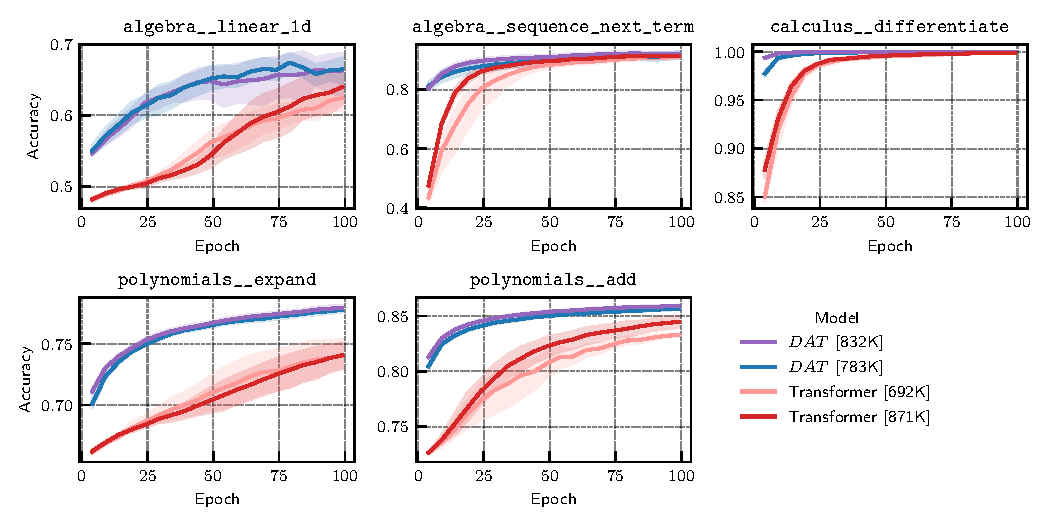
\includegraphics[width=0.8\textwidth]{figs/experiments/math/math_training_curves_interpolation.pdf}
    \caption{Validation accuracy over the course of training for seq2seq mathematical problem-solving.}
\end{figure}

\begin{table}
    \centering
    \caption{Sequence-to-sequence symbolic mathematical processing. Comparison to Transformer at multiple scales. \textit{DAT} models have model dimension $128$ and Transformer models have model dimension $144$, with three models each with 2, 3, or 4 layers. Superiority of \textit{DAT} persists across all depths and model sizes.}
    \begin{tabular}{l|l|cc}
\toprule
Task & Model &  Accuracy \\
\midrule
\multirow{7}{*}{$\texttt{algebra\_\_linear\_1d}$} & Transformer [692K] &                    62.5\% \\
                                 & $DAT$ [783K] &                    66.5\% \\
                                 & Transformer [871K] &                    64.0\% \\
                                 & $DAT$ [1.09M] &                    76.6\% \\
                                 & Transformer [1.3M] &                    64.3\% \\
                                 & $DAT$ [1.43M] &                    74.7\% \\
                                 & Transformer [1.7M] &                    50.9\% \\
\cline{1-3}
\multirow{7}{*}{$\texttt{algebra\_\_sequence\_next\_term}$} & Transformer [692K] &                    91.1\% \\
                                 & $DAT$ [783K] &                    91.6\% \\
                                 & Transformer [871K] &                    91.4\% \\
                                 & $DAT$ [1.09M] &                    97.3\% \\
                                 & Transformer [1.3M] &                    96.9\% \\
                                 & $DAT$ [1.43M] &                        -- \\
                                 & Transformer [1.7M] &                    82.6\% \\
\cline{1-3}
\multirow{7}{*}{$\texttt{calculus\_\_differentiate}$} & Transformer [692K] &                    99.9\% \\
                                 & $DAT$ [783K] &                   100.0\% \\
                                 & Transformer [871K] &                    99.9\% \\
                                 & $DAT$ [1.09M] &                        -- \\
                                 & Transformer [1.3M] &                    99.9\% \\
                                 & $DAT$ [1.43M] &                   100.0\% \\
                                 & Transformer [1.7M] &                   100.0\% \\
\cline{1-3}
\multirow{7}{*}{$\texttt{polynomials\_\_add}$} & Transformer [692K] &                    83.3\% \\
                                 & $DAT$ [783K] &                    85.6\% \\
                                 & Transformer [871K] &                    84.5\% \\
                                 & $DAT$ [1.09M] &                    87.9\% \\
                                 & Transformer [1.3M] &                    86.9\% \\
                                 & $DAT$ [1.43M] &                    88.7\% \\
                                 & Transformer [1.7M] &                    87.3\% \\
\cline{1-3}
\multirow{7}{*}{$\texttt{polynomials\_\_expand}$} & Transformer [692K] &                    74.0\% \\
                                 & $DAT$ [783K] &                    77.8\% \\
                                 & Transformer [871K] &                    74.1\% \\
                                 & $DAT$ [1.09M] &                        -- \\
                                 & Transformer [1.3M] &                        -- \\
                                 & $DAT$ [1.43M] &                    92.2\% \\
                                 & Transformer [1.7M] &                    87.2\% \\
\bottomrule
\end{tabular}

\end{table}

% choose either table or figure
% NOTE: maybe the table would be better to include than this fig? or not? the table makes the numbers transparent and exposes the details of the architectural configurations.
\begin{figure}[ht]
    \begin{subfigure}{0.44\textwidth}
        \centering
        \captionsetup{width=.9\linewidth}
        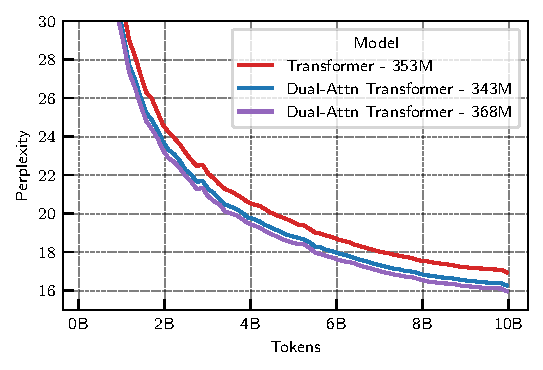
\includegraphics[width=\textwidth]{figs/experiments/fineweb/350M_scale_lm.pdf}
        \caption{350M parameter scale ($\dmodel = 1024$, $\nlayers = 24$)}
    \end{subfigure}
    \begin{subfigure}{0.44\textwidth}
        \centering
        \captionsetup{width=.9\linewidth}
        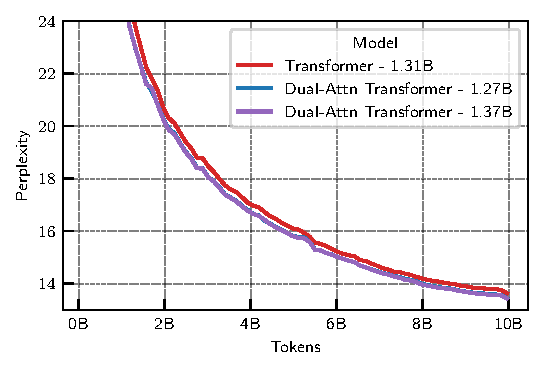
\includegraphics[width=\textwidth]{figs/experiments/fineweb/1_3B_scale_lm.pdf}
        \caption{1.3B parameter scale ($\dmodel = 2048$, $\nlayers = 24$)}
    \end{subfigure}
    \caption{Perplexity curves on language modeling with the fineweb dataset. The $x$-axis indicates the number of tokens and the $y$-axis is the validation perplexity. \textit{DAT} learns faster and achieves smaller perplexity at multiple model size scales.}\label{fig:tiny_stories_val_loss_curves}
\end{figure}

\begin{table}[]
    \centering
    \caption{Language Modeling on Fineweb dataset.}\label{tab:my-table}
    % \resizebox{\textwidth}{!}{%
    % \begin{tabular}{@{}l|ccccccc|c@{}}
    \begin{tabular}{@{}l|c|cccccc|c@{}}
    \toprule
    Model / Param count   & \# Tokens &$\dmodel$&$\nlayers$& $\nhsa$  & $\nhra$ & $d_r$ & $n_{kv}^{h}$ & Perplexity $\downarrow$ \\ \midrule\hline
    Transformer - 353M    & 10B       & 1024    & 24       & 16       & -        & -     & -           & 16.94     \\
    \textit{DAT} - 343M   & 10B       & 1024    & 24       & 8        & 8        & 32    & 4           & 16.26     \\
    \textit{DAT} - 368M   & 10B       & 1024    & 24       & 8        & 8        & 32    & 8           & 15.97     \\\midrule
    Transformer - 1.31B   & 10B       & 2048    & 24       & 32       & -        & -     & -           & 13.63     \\
    \textit{DAT} - 1.27B  & 10B       & 2048    & 24       & 16       & 16       & 64    & 8           & 13.44     \\
    \textit{DAT} - 1.37B  & 10B       & 2048    & 24       & 16       & 16       & 64    & 16          & 13.43     \\ \bottomrule
    % Model / Param count   &$\dmodel$&$\nlayers$& $\nhsa$  & $\nhra$ & $n_r$ & $n_{kv}^{h}$ & Perplexity $\downarrow$ \\ \midrule\hline
    % Transformer - 353M   & 1024    & 24       & 16       & -        & -     & -           & 16.944     \\
    % \textit{DAT} - 343M  & 1024    & 24       & 8        & 8        & 32    & 4           & 16.258     \\
    % \textit{DAT} - 368M  & 1024    & 24       & 8        & 8        & 32    & 8           & 15.969     \\\midrule
    % Transformer - 1.31B  & 2048    & 24       & 32       & -        & -     & -           & 13.630     \\
    % \textit{DAT} - 1.27B & 2048    & 24       & 16       & 16       & 64    & 8           & 13.440     \\
    % \textit{DAT} - 1.37B & 2048    & 24       & 16       & 16       & 64    & 16          & 13.426     \\ \bottomrule
    \end{tabular}%
    % }
    % & $n_s$ 
    % & -     
    % & 1024  
    % & 1024  
    % & -     
    % & 512   
    % & 2048  
\end{table}

\end{document}